\section{数据校验}

\subsection{下载工具}
\begin{frame}
    从gitee下载最新版的订单检查工具,以1.0.0版本为例

    {\small\url{https://gitee.com/zhengxueke/check-laads-order/releases}}

    \begin{annotationimage}{width=\linewidth}{images/3.1下载工具.jpg}
        \draw[red,very thick](0.3,0.16) rectangle (0.56,0.2);
    \end{annotationimage}
\end{frame}
\begin{frame}
    \frametitle{解压文件}
    下载好的压缩包,一定要全部解压缩到本地文件夹后再操作。

    解压后如图

    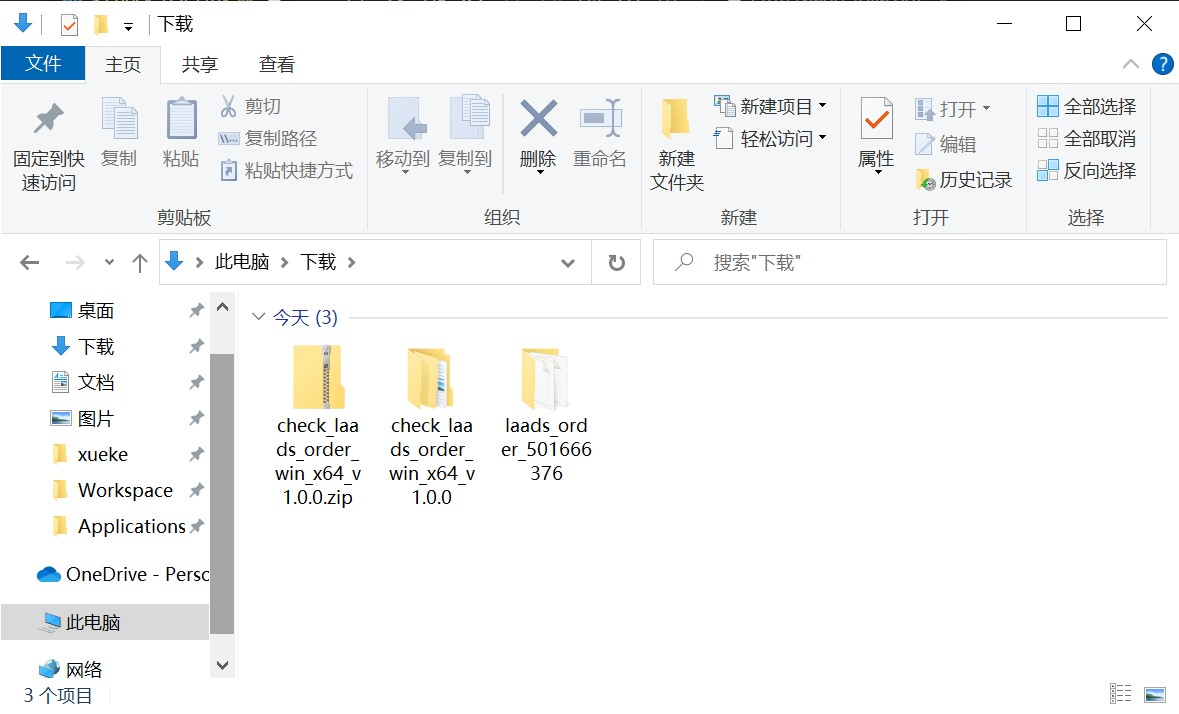
\includegraphics[width=\linewidth]{images/3.2解压}
\end{frame}
\subsection{执行校验}
\begin{frame}
    \frametitle{找到程序}
打开check\_laads\_order.exe主应用程序

    \begin{annotationimage}{width=\linewidth}{images/3.3找到程序}
\draw[red,very thick](0.22,0.24) rectangle (0.42,0.3);
    \end{annotationimage}
\end{frame}
\begin{frame}
    \frametitle{导入订单位置}
\end{frame}
\subsection{重新下载问题文件}
\begin{frame}
    \frametitle{校验结果}
\end{frame}
\frametitle{打开校验程序}
\begin{frame}
    \frametitle{重新下载}
\end{frame}



